\chapter{机器学习的基础理论}\label{chap:ml_theory}

\section{引言}

本章节主要对机器学习的基础理论进行简要介绍,不仅包含各种算法(线性回归、$k$NN算法、SVR、决策树、随机森林、LSTM-RNN和CNN),还包含了优化算法、模型泛化能力、性能度量指标等。

本质上说,各类算法的初衷是为解决某一特定问题而进行开发的。若想将某一种算法迁移到其他问题中,可能需要再次耗费大量的经历重新修缮算法。与之不同的是,机器学习算法可以从大量样本中训练算法。若想将训练好的算法迁移到其他类似问题上,只需要在原算法的基础上再进行稍微调整训练。因此,即使面临的问题有所差异,但学到的模型具有一定的通用性\citep{Goodfellow2016Deep}。

一般地,机器学习可以分为三类,分别为监督学习、无监督学习和半监督学习。监督学习算法的数据集具有标签,无监督学习算法的数据集没有标签,半监督学习算法则自我利用未被标记样本来提升模型性能。本文的研究目标将重点集中在监督学习的应用上。文中被标记的数据部分来自实际观测点结果,部分来自数值模拟的结果。基于这些被标记的数据集,使用监督学习算法,可以将数据中隐藏的信息挖掘出来建立模型,从而能够利用评估良好的模型预测未来的情况。

传统的机器学习从训练样本出发,试图通过数据本身而不是原理分析获得规律,实现对未来数据行为或趋势的准确预测。相关的机器学习算法大致包括线性回归、$k$NN算法、SVR、决策树、随机森林等。这些机器学习方法通过平衡学习结果的有效性与学习模型的可解释性,为解决有限样本的学习问题提供了一种框架,可用于有限样本情况下的模式分类、回归分析、概率密度估计、聚类等。这些机器学习方法共同的重要理论基础之一是统计学。

深度学习,又称深度神经网络(超过3层的神经网络),是机器学习中发展最迅速的一个子领域。深度学习通过在输入层和输出层之间使用隐藏层对数据的中间表征进行建模,这一点其他算法很难做到。深度学习中的卷积计算、池化计算、dropout等方法可以有效减少数据维度。这样做的前提是,需要输入大量的数据,估算更多的参数,同时需要强大的计算能力。实际应用过程中,在小样本数据下,深度学习的性能不一定能超过传统意义上的机器学习方法,诸如支持向量机。

在本章中,我们首先介绍机器学习中的各种算法(第~\ref{sec:机器学习各种算法介绍}节),包括线性回归(第~\ref{sec:线性回归}节)、$k$NN算法(第~\ref{sec:k近邻算法}节)、SVR~\ref{sec:支持向量回归}节)、决策树(第~\ref{sec:决策树}节)、随机森林(第~\ref{sec:随机森林}节)、LSTM-RNN(第~\ref{sec:LSTM-RNN}节)和CNN(第~\ref{sec:卷积神经网络}节)。随后,我们介绍参数化模型的相关优化原理(第\ref{sec:机器学习模型的优化}节)。通过深入理解机器学习的原理以及训练必备的条件,为这些模型的构建和开发提供基础。


\section{机器学习各种算法介绍}\label{sec:机器学习各种算法介绍}

在本节,我们会简要介绍机器学习算法的基本概念和本文所涉及的机器学习方法。首先,机器学习是从数据中提取知识。或者说,机器学习算法是一种能够从数据中学习经验的算法。~\citet{Mitchell1997Machine}给机器学习提供了一个形式化的定义:``假设性能$P$用来评估计算机计算的某类任务$T$,若该计算利用经验$E$在任务$T$上性能$P$有所提升,则对于$T$和$P$而言,计算机程序从$E$进行了学习。''

假定数据集为$D=\{(\Vector{x}_1,y_1),(\Vector{x}_2,y_2),\ldots,(\Vector{x}_m,y_m)\}$,其中$\Matrix{X}=\{\Vector{x}_1,\Vector{x}_2,\ldots,\Matrix{x}_m\}$为输入向量,$\Vector{x}_i\in\mathcal{X}$为特征空间,$\Vector{Y}=\{y_1,y_2,\ldots,y_m\}$为输出向量,$y_i\in\mathcal{Y}$为输出特征空间。一般地,我们抽取数据集$D$中的部分数据作为训练集,学习到一个从输入空间$\mathcal{X}$到输出空间$\mathcal{Y}$的映射$f:\mathcal{X}\rightarrow\mathcal{Y}$。通过该映射(模型),使用未经训练的数据(即测试数据集)进行测试。测试过程中需要考虑性能度量的指标。需要注意的是,机器学习关注的是使模型能够很好地适用于测试机,而不仅仅在训练集中表现良好,这就要求模型具有泛化(generalization)能力。


\subsection{线性回归}\label{sec:线性回归}

线性回归(linear regression,简写为LR)是机器学习中很多算法的基本思想,是一种经典的、简单的回归模型,其用来预测的结果是连续变量。线性回归许多非线性模型均是在机器学习模型的基础上通过引入高维映射或层级结构演化而来。假定数据集为$D=\{(\Vector{x}_1,y_1),(\Vector{x}_2,y_2),\ldots,(\Vector{x}_m,y_m)\}$,其中$\Matrix{X}=\{\Vector{x}_1,\Vector{x}_2,\ldots,\Matrix{x}_m\}$是输入特征空间,$\Vector{Y}=\{y_1,y_2,\ldots,y_m\}$是输出特征空间。线性回归的主要目的是学习一个函数$f(\Matrix{X})$(公式~\ref{eq:lr_fun}),使得$f(\Matrix{X})$与目标值$\Vector{Y}$之间的偏差尽可能地小。
\begin{equation}
  \label{eq:lr_fun}
  f(\Matrix{X})=\Matrix{W}^{\text{T}}\Matrix{X}+\Vector{b}.
\end{equation}
其中,$\Matrix{W}$和$\Vector{b}$都是待定的模型参数。确定$\Matrix{W}$和$\Vector{b}$的关键在于衡量$f(\Matrix{X})$与$\Vector{Y}$之间的距离,均方差(mean square error, 简写为MSE,见式~\ref{eq:mse})是最常用的距离度量工具。这里试图让MSE最小化,即
\begin{equation}
  \label{eq:mse}
  \text{MSE}=\frac{1}{m}\sum_{i=1}^{m}(f(\Vector{x}_i)-y_i)^2.
\end{equation}
这里将$\Matrix{W}$和$\Vector{b}$合并成向量$\hat{\Matrix{W}}=(\Matrix{W};\Vector{b})$。根据\ref{eq:mse},代价函数(优化目标)可写成
\begin{equation}
  \label{eq:lr_loss}
  J(\hat{\Matrix{W}})=\min_{\hat{\Matrix{W}}}\sum_{i=1}^{m}(f(\Vector{x}_i)-y_i)^2.
\end{equation}

线性回归适合强相关性的数据集。思想简单,结果易解释,拟合模型的速度快。更为重要的一点是,不需要调参。但缺点也显而易见,线性回归模型不适合非线性数据集。当样本特征很多,而样本数相对较少时,式~\ref{eq:lr_loss}容易陷入过拟合。在线性回归的基础上加上正则项,可以有效消除多重共线性特征的影响,在一定程度上规避了过拟合问题。可对
式~\ref{eq:lr_loss}引入了正则化项。若使用$L_2$范数正则化,则有
\begin{equation}
  \label{eq:lr_loss_ridge}
  J(\hat{\Matrix{W}})=\min_{\hat{\Matrix{W}}}\sum_{i=1}^{m}(f(\Vector{x}_i)-y_i)^2+\lambda\left\|\hat{\Matrix{W}}\right\|_2^2.
\end{equation}
其中,正则化参数$\lambda>0$。式~\ref{eq:lr_loss_ridge}亦称岭回归(ridge regression)。若使用$L_1$范数正则化,则有
\begin{equation}
  \label{eq:lr_loss_lasso}
  J(\hat{\Matrix{W}})=\min_{\hat{\Matrix{W}}}\sum_{i=1}^{m}(f(\Vector{x}_i)-y_i)^2+\lambda\left\|\hat{\Matrix{W}}\right\|_1.
\end{equation}
其中,正则化参数$\lambda>0$。式~\ref{eq:lr_loss_ridge}亦称LASSO(least absolute shrinkage and selection operator)。

利用最小二乘法对$\Matrix{W}$和$\Vector{b}$进行估计。则有
\begin{equation}
  \label{eq:lr_wb}
  \hat{\Matrix{W}}^*=\mathop{\arg\min}\limits_{\hat{\Matrix{W}}}(\Vector{Y}-(\Matrix{X};\Vector{I})\hat{\Matrix{W}})^{\text{T}}(\Vector{Y}-(\Matrix{X};\Vector{I})\hat{\Matrix{W}}).
\end{equation}
令$E_{\hat{\Matrix{W}}}={\hat{\Matrix{W}}}(\Vector{Y}-(\Matrix{X};\Vector{I})\hat{\Matrix{W}})^{\text{T}}(\Vector{Y}-(\Matrix{X};\Vector{I})\hat{\Matrix{W}})$,对$\hat{\Matrix{W}}$求导得到
\begin{equation}
  \label{eq:lr_wb_partial}
  \frac{\partial{E_{\hat{\Matrix{W}}}}}{\partial{\hat{\Matrix{W}}}}=2(\Matrix{X};\Vector{I})^{\text{T}}((\Matrix{X};\Vector{I})\hat{\Matrix{W}})-\Vector{Y}).
\end{equation}
令式~\ref{eq:lr_wb_partial}为零,可得$\hat{\Matrix{W}}$最优解的封闭式。

\subsection{k近邻算法}\label{sec:k近邻算法}

$k$近邻(k-nearest neighbors,简称$k$NN)算法非常简单且高效,是一种常用的监督学习方法。其工作机制可描述为:给定测试样本,基于某种度量找出训练集中与其最靠近点$k$个训练样本,再基于这$k$个样本的信息进行预测。在分类问题中,使用投票法(利用$k$个样本中出现最多的样本类别作为预测结果)。在回归问题中,可以使用平均值法(利用$k$个样本的实际值的平均作为最终的预测结果)。这两类问题也可以基于距离远近进行加权平均或加权投票。$k$NN算法的关键在于$k$值的选择、距离度量和决策规则。$k$NN模型在训练时会一次性输入整个训练数据集,因此需要大量内存或空间来存储所有数据。$k$NN模型在高维情况下,容易出现样本稀疏、距离计算困难等问题,即维数灾难。

在训练集中数据和标签已知的情况下,输入测试样本,将测试样本的特征与训练集中对应的特征进行相互比较,找到训练集中与之最为相似的前$k$个样本,则该测试样本对应的类别就是$k$个数据中出现次数最多的那个分类。$k$NN算法描述为:
\begin{enumerate}
\item 计算测试数据与各个训练样本之间的距离;
\item 按照距离的递增关系进行排序;
\item 选取距离最小的$k$个样本;
\item 确定前$k$个样本所在类别的出现频率;
\item 返回前$k$个样本中出现频率最高的类别作为测试样本的预测分类。
\end{enumerate}

\subsection{决策树}\label{sec:决策树}

决策树(decision tree)根据处理数据类型的不同,可分为分类决策树核回归决策树树(regression decision tree,简称RDT。分类决策树可用于处理离散型数据,回归决策树可用于处理连续性数据。决策树由节点核有向边组成。一棵决策树包含一个根节点、若干个内部节点和若干个叶节点。根节点包含整个样本集$\Matrix{X}$,内部节点表示特征或属性,叶节点对应于决策结果。

在进行分类或回归任务时,从根节点开始,对样本的某一属性判定测试,根据测试结果划分到子节点;这时每个子节点对应着该特征的一个取值,将这个过程不断重复,直至目标到达叶节点。本质上,决策树是将空间超平面进行划分的一种方法。每分割一次,都会将当前的空间根据属性的取值进行划分,从而使得每一个叶节点在空间中不相交。决策树学习的目的是为了得到一棵泛化能力强的决策树。

假设给定数据集$D=\{(\Vector{x}_1,y_1),(\Vector{x}_2,y_2),\ldots,(\Vector{x}_m,y_m)\}$,$\Matrix{X}$和$\Vector{Y}$分别为输入和输出特征空间,则$\Matrix{X}=\{\Vector{x}_1,\Vector{x}_2,\ldots,\Matrix{x}_m\}$,$\Vector{Y}=\{y_1,y_2,\ldots,y_m\}$。决策树的基本流程遵循分而治之(divide-and-conquer)的策略,见算法~\ref{alg:decision_tree}。决策树的生成过程是递归的。在决策树中,有以下三种情况会出现递归返回:(1)当前节点包含的样本全属于同一类别,不需要进行划分(见算法~\ref{alg:decision_tree}中的第\ref{alg:decision_tree_if1})行;(2)当前属性集为空,或是所有样本在所有属性上取值均相等,无法划分(见算法~\ref{alg:decision_tree}中的第\ref{alg:decision_tree_if2}行);(3)当前节点包含的样本集合为空,不能划分(见算法~\ref{alg:decision_tree}中的第\ref{alg:decision_tree_if3}行)。
\begin{algorithm}[!htbp]
  \small
  \caption{决策树学习基本算法}\label{alg:decision_tree}
  \textbf{Input}:{数据集$D=\{(\Vector{x}_1,y_1),(\Vector{x}_2,y_2),\ldots,(\Vector{x}_m,y_m)\}$;属性集$A=\{a_1,a_2,\ldots,a_d\}$.}
  \begin{algorithmic}[1]
    \Procedure{Tree}{$D,A$}
    \State 生成节点Node;
    \If{数据集$D$中的所有样本属于同一类别$C$,即$D\subset C$}
    \State 将Node标记为$C$类叶节点;\textbf{return}\label{alg:decision_tree_if1}
    \EndIf
    \If{$A=\emptyset$ \textbf{OR} $D$中样本在$A$上取值相同}
    \State 将Node标记为叶节点,其类别标记为$D$中样本数量最多的类;\textbf{return}\label{alg:decision_tree_if2}
    \EndIf
    \State 从$A$中选择最优划分属性$a^*=\{a_1^*,a_2^*,\ldots,a_v^*\}$;
    \For{$a_i^* (i\in\{1,2,\ldots,v\})$}
      \State 在Node下再生成一个分支;$D_v$表示$D$在$a^*$上取值为$a_v^*$的样本子集;
      \If{$D_v=\emptyset$}
      \State 将分支节点标记为叶节点,其类别标记为$D$中样本最多的类;\textbf{return} \label{alg:decision_tree_if3}
      \Else{以Tree$(D_v,A,\{a^*\})$为分支节点}
      \EndIf 
    \EndFor
    \EndProcedure
  \end{algorithmic}
  \textbf{Output}:{输出最优决策树Tree$(D,A)$.}
\end{algorithm}

在算法~\ref{alg:decision_tree}中,决策树学习的关键是确定划分最优属性以及叶节点的属性值。整体上,随着划分过程不断推进,决策树的分支节点所包含的样本尽可能属于同一类别,即节点的纯度越来越高。假设将输入空间$\Matrix{X}$划分为$H$个单元$R_1,R_2,\ldots,R_H$,并且在每个单元$R_h$上有一个固定的输出值$c_m$,回归树模型表示为
\begin{equation}
  \label{eq:decision_tree}
  f(\Matrix{X})=\sum_{h=1}^{H}c_hI.
\end{equation}

当空间划分确定时,可用平方误差$\sum_{\Vector{x}_i\in R_h}(y_i-f(\Vector{x}_i))^2$表示回归树对于训练数据集的误差,最小化平方误差可求得每个单元上的最优输出值。易得到,$c_h$的最优值$\hat{c}_h$,是单元$R_h$上所有样本$\Vector{x}_i$对应的输出$y_i$的均值(见式)。
\begin{equation}
  \label{eq:decision_tree_unit}
  \hat{c}_h=\text{mean}(y_i|\Vector{x}_i\in R_h).
\end{equation}

本研究中采用CART决策树对输入空间$\Matrix{X}$进行划分,选择第$k$个样本$\Vector{x}_k$和其值$s$分别作为切分变量和切分点。定义两个区域$R_1(j,s)=\{\Matrix{x}|\Vector{x}_k\le s\}$和$R_2(j,s)=\{\Matrix{x}|\Vector{x}_k>s\}$,然后寻找最优切分变量$\Vector{x}_k$和最优切分点$s$,详情见式~\ref{eq:decision_tree_split}。
\begin{equation}
  \label{eq:decision_tree_split}
  \min_{k,s}=\Bigg[\min_{c_1}^{}\sum_{x_i\in R_1(k,s)}(y_i-c_1)^2+\min_{c_2}^{}\sum_{x_i\in R_2(k,s)}(y_i-c_2)^2\Bigg].
\end{equation}

用选定的最优切片样本$k$和最优切分点$s$划分区域并决定响应的输出值:$\hat{c}_1=\text{mean}(y_i|\Vector{x}_i\in R_1(j,s))$和$\hat{c}_2=\text{mean}(y_i|\Vector{x}_i\in R_2(j,s))$。依次将输入空间划分为两个区域,直到不能划分为止。


\subsection{随机森林}\label{sec:随机森林}
随机森林(random forest,简称RF)是一种由多个决策树组成的集成算法,是Bagging(bootstrap AGGregatING)的一种扩展变体。RF中不同决策树之间并没有关联性。通过组合多个决策树(这里也称弱分类器),最终结果通过投票或取均值,使得整体模型的结果具有较高的精确度和泛化性能。RF有两个关键特性,``随机''和``森林''。``随机''使RF具有抗过拟合能力。``森林''指的是多个决策树组成在一起,其实这是RF拟合能力强大的原因。

假设给定数据集$D=\{(\Vector{x}_1,y_1),(\Vector{x}_2,y_2),\ldots,(\Vector{x}_m,y_m)\}$,$\Matrix{X}$和$\Vector{Y}$分别为输入和输出特征空间,则$\Matrix{X}=\{\Vector{x}_1,\Vector{x}_2,\ldots,\Matrix{x}_m\}$,$\Vector{Y}=\{y_1,y_2,\ldots,y_m\}$。构造随机森林需要四步,见算法~\ref{alg:random_forest}。详细过程可描述为:

\begin{enumerate}
\item 一个样本容量为$N$的样本,有放回的抽取$N$次,每次抽取1个,最终形成了$N$个样本。这选择好了的$N$个样本用来训练一个决策树,作为决策树根节点处的样本。这个过程也被称作自助采样法(bootstrap sampling);
\item 当每个样本有$M$个属性时,在决策树的每个节点需要分裂时,随机从这$M$个属性中选取出$m$个属性,满足条件$<<mM$。然后从这$m$个属性中采用某种策略(比如说信息增益)来选择1个属性作为该节点的分裂属性;
\item 决策树形成过程中每个节点都要按照步骤2来分裂。如果下一次该节点选出来的那一个属性是刚刚其父节点分裂时用过的属性,则该节点已经达到了叶子节点,无须继续分裂。若属性不能再分裂,则形成了决策树;
\item 按照步骤1~3建立大量的决策树,这样就构成了随机森林了。
\end{enumerate}

\begin{algorithm}[!htbp]
  \small
  \caption{RF基本算法}\label{alg:random_forest}
  \textbf{Input}:{数据集$D=\{(\Vector{x}_1,y_1),(\Vector{x}_2,y_2),\ldots,(\Vector{x}_m,y_m)\}$;属性集$A=\{a_1,a_2,\ldots,a_d\}$.}
  \begin{algorithmic}[1]
    \Procedure{RF}{$D,A$}
    \State 随机抽样,训练决策树;
    \While{节点可以分裂}
      \State 随机选取属性,做节点分裂属性;\textbf{return}
    \EndWhile
    \State 建立大量决策树,形成森林。
    \EndProcedure
  \end{algorithmic}
  \textbf{Output}:{输出最优随机森林RF$(D,A)$.}
\end{algorithm}


\subsection{支持向量回归}\label{sec:支持向量回归}

支持向量回归(support vector regression,简写为SVR)属于典型的监督学习算法之一。假定数据集为$D=\{(\Vector{x}_1,y_1),(\Vector{x}_2,y_2),\ldots,(\Vector{x}_m,y_m)\}$,其中$\Matrix{X}=(\Vector{x}_1,\Vector{x}_2,\ldots,\Matrix{x}_m)$是输入特征空间,$\Matrix{Y}=(y_1,y_2,\ldots,y_m)$是输出特征空间。线性回归的主要目的是学习一个函数$f(\Matrix{X})$(公式~\ref{eq:svr_fun}),使得$f(\Matrix{X})$与目标值$\Vector{Y}$之间的偏差尽可能地小,$\Matrix{W}$和$\Vector{b}$都是待定的模型参数。
\begin{equation}
  \label{eq:svr_fun}
  f(\Matrix{X})=\Matrix{W}^{\text{T}}\Matrix{X}+\Vector{b}
\end{equation}

传统回归模型计算损失通常直接通过模型输出$f(\Matrix{X})$与目标值$\Vector{Y}$之间的距离,当且仅当$f(\Matrix{X})-\Vector{Y}=\Matrix{0}$时,损失才为0。事实上,在很多现实情况中,误差在一定的范围内是被容忍的。而SVR真是基于这一点,假设$f(\Matrix{X})-\Vector{Y}\le \epsilon$,当$f(\Matrix{X})$与$\Vector{Y}$之间的距离大于$\epsilon$时,需要计算损失。于是,SVR问题可形式化为
\begin{equation}
  \label{eq:svr_min}
  \begin{split}
  \min\limits_{\Matrix{W},\Vector{b}}\frac{1}{2}\left\|\Matrix{W}\right\|^{2}+C\sum_{i=1}^{m}\mathscr{l}_{\epsilon}(f(\Vector{X}_i)-y_i),\\
  s.t.  
  |f(\Matrix{X})-(\Matrix{W}^{T}\Matrix{X}+\Vector{b})|\le \epsilon
  \end{split}
\end{equation}
其中$C$为正则化常数,$\mathscr{l}_{\epsilon}$为$\epsilon$-不敏感损失函数。
\begin{equation}
  \label{eq:svr_loss}
  \mathscr{l}_{\epsilon}(z)=
  \begin{cases}
    0,\qquad\quad \text{if}\quad |z|\le \epsilon;\\
    |z|-\epsilon,\quad \text{otherwise}.
  \end{cases}
\end{equation}

这里引入两个松弛变量$\varepsilon_i$和$\hat{\varepsilon}_i$,式~\ref{eq:svr_min}可改写为
\begin{equation}
  \label{eq:svr_min_v2}
  \begin{split}
  \min\limits_{\Matrix{W},\Vector{b},\epsilon_i,\hat{\epsilon}_i}\frac{1}{2}\left\|\Matrix{W}\right\|^{2}+C\sum_{i=1}^{m}(\varepsilon_i+\hat{\varepsilon}_i),\\
  s.t. 
  \begin{cases}
  |f(\Vector{x}_i)-(\Matrix{W}_i^{T}\Vector{x}_i+b_i)|\le \varepsilon_i+\hat{\varepsilon}_i,\\
  \varepsilon_i\ge 0, \hat{\varepsilon}_i\ge 0, i=1,2,\ldots,m.
  \end{cases}
  \end{split}
\end{equation}

引入拉格朗日乘子$\mu_i,\hat{\mu}_i,\alpha_i,\hat{\alpha}_i\ge 0$,从而得到拉格朗日函数
\begin{equation}
  \label{eq:svr_lagrange}
  \begin{split}
  L(\Matrix{W},\Vector{b},\Vector{\epsilon},\Vector{\hat{\epsilon}},\Vector{\mu},\Vector{\hat{\mu}},\Vector{\alpha},\hat{\Vector{\alpha}})=\frac{1}{2}\left\|\Matrix{W}\right\|^{2}+C\sum_{i=1}^{m}(\varepsilon_i+\hat{\varepsilon}_i)-\sum_{i=1}^{m}(\mu_{i}\varepsilon_i+{\hat{\mu}_i\varepsilon}_i)\\
  +\sum_{i=1}^{m}\alpha_i(f(\Vector{x}_i)-y_i-(\epsilon_i+\varepsilon_i))+\sum_{i=1}^{m}\hat{\alpha}_i(f(\Vector{x}_i)-y_i-(\epsilon_i+\hat{\varepsilon}_i)).
  \end{split}
\end{equation}

对式~\ref{eq:svr_lagrange}分别进行求$\Matrix{W},\Vector{b},\epsilon_i,\hat{\varepsilon}_i)$的偏导,并将结果整合到式~\ref{eq:svr_lagrange}中,得到SVR的对偶问题
\begin{equation}
  \label{eq:svr_dual}
  \begin{split}
  \max\limits_{\Vector{\alpha},\hat{\Vector{\alpha}}}\sum_{i=1}^{m}[y_i(\hat{\alpha}_i-\alpha_i)-\epsilon(\hat{\alpha}_i+\alpha_i)]-\frac{1}{2}\sum_{i=1}^{m}\sum_{j=1}^{m}(\hat{\alpha}_i-\alpha_i)(\hat{\alpha}_j-\alpha_j)\Vector{x}_i^{\text{T}}\Vector{x}_j,\\
  s.t. 
  \sum_{j=1}^{m}(\hat{\alpha}_i-\alpha_i)=0, \quad \alpha_i, \hat{\alpha}_i\in[0,C].
  \end{split}
\end{equation}

以上过程需要满足Karush-Kuhn-Tucker(KKT)条件,即
\begin{equation}
  \label{eq:svr_kkt}
  \begin{cases}
    \alpha_i(f(\Vector{x}_i-y_i-\epsilon_i-\varepsilon_i))=0,\\
    \hat{\alpha}_i(f(\Vector{x}_i-y_i-\epsilon_i-\hat{\varepsilon}_i))=0,\\
    \alpha_i\hat{\alpha}_i=0,\quad  \varepsilon_i\hat{\varepsilon}_i=0,\\
    (C-\alpha_i)\hat{\varepsilon}_i=0,\quad  (C-\alpha_i)\hat{\varepsilon}_i=0.
  \end{cases}
\end{equation}
可以看出,当且仅当$f(\Vector{x}_i-y_i-\epsilon_i-\varepsilon_i)=0$时,$\alpha_i=0$;当且仅当$f(\Vector{x}_i-y_i-\epsilon_i-\hat{\varepsilon}_i)=0$时,$\hat{\alpha}_i=0$。也就是说,在样本$(\Vector{x}_y,y_i)$没有在$\epsilon$间隔带中,$\alpha_i=0$和$\hat{\alpha}_i=0$才能取非零值。此外,$f(\Vector{x}_i-y_i-\epsilon_i-\varepsilon_i)=0$和$f(\Vector{x}_i-y_i-\epsilon_i-\hat{\varepsilon}_i)=0$两者只能有一个成立,因此$\alpha_i$和$\hat{\alpha}_i$至少有一个为零。

为了增强SVR的非线性特征,我们考虑将$\Matrix{X}$映射到高维空间。但SVR的性能更多地取决于样本之间的距离。因此,SVR使用核函数替代高维空间映射。
\begin{equation}
  \label{eq:svr_kernel}
   \mathcal{k}(\Vector{x}_i,\Vector{x}_j)=\phi(\Vector{x}_i)^{\text{T}}\phi(\Vector{x}_j)
\end{equation}

式\ref{eq:svr_dual}可转化为
\begin{equation}
  \label{eq:svr_dual_kernel}
  \begin{split}
  \max\limits_{\Vector{\alpha},\hat{\Vector{\alpha}}}\sum_{i=1}^{m}[y_i(\hat{\alpha}_i-\alpha_i)-\epsilon(\hat{\alpha}_i+\alpha_i)]-\frac{1}{2}\sum_{i=1}^{m}\sum_{j=1}^{m}(\hat{\alpha}_i-\alpha_i)(\hat{\alpha}_j-\alpha_j)\mathcal{k}(\Vector{x}_i,\Vector{x}_j),\\
  s.t. 
  \sum_{j=1}^{m}(\hat{\alpha}_i-\alpha_i)=0, \quad \alpha_i, \hat{\alpha}_i\in[0,C].
  \end{split}
\end{equation}

在非线性情况中,最优问题在特征空间(而不是输入空间)中函数需要满足可微条件。最终SVR可表示为
\begin{equation}
  \label{eq:svr_kernel_v2}
  f(\Matrix{X})=\sum_{i=1}^{m}(\hat{\alpha}_i-\alpha_i)\mathcal{k}(\Vector{x}_i,\Vector{x}_j)+\Vector{b}.
\end{equation}
在下文的研究中,我们选择了线性核函数,公式表达如下
\begin{equation}
  \label{eq:svr_kernel_linear}
  \mathcal{k}(\Vector{x}_i,\Vector{x}_j)=\Vector{x}_i^{\text{T}}\Vector{x}_j.
\end{equation}



\subsection{卷积神经网络}\label{sec:卷积神经网络}

在人工智能领域,神经网络(artificial neural network,简写为ANN)应用最为广泛,因其能拟合非常复杂的函数。至此,ANN有了两大模型,即全连接网络以及卷积神经网络(convolution neural network,可简写为CNN)。目前很多研究都关注二维卷积神经网络(two-dimensional CNNs,简写为2D-CNN),尤其是在图像识别、自动驾驶等领域。而一维卷积神经网络(one-dimensional CNN,简写为1DCNN)只在序列数据上有所涉及,比如自然语言处理、信号处理等。

一般来讲,CNN有两大特点。第一,CNN能够有效较大的数据形状压缩为较小的形状。第二,在压缩形状的同时,还能有效地保留图片特征。典型的CNN由三部分组成,分别为卷积层、池化层和全连接层。卷积层负责提取图像中的局部特征;池化层用来大幅度降低参数量级(降维),防止出现过拟合;全连接层类似于传统神经网络的层,用来输出最终结果。

卷积层的运算过程可理解为使用一个卷积核来过滤原始数据中的部分小区域,从而得到这些小区域的特征值。在具体应用中,卷积核可以有多个。一般认为,每个卷积核代表了一种特征模式。如果某个区域与此卷积核的卷积和较大,则该区块十分接近与该卷积核。可以说,卷积层通过卷积核的过滤提取小区域中的特征。

池化层,也称作下采样层,主要用来降低数据的维度(形状)。常见的池化运算包括最大池化和平均池化。之所以加入池化层,是因为当仅仅加入卷积层时,所得到的特征图的维度可能依旧很大。池化层相比与卷积层而言,能够更加有效地降低数据维度,这么做不但可以大大减少运算量,还可以有效避免过拟合。

CNN的输出层多数情况下都为全连接层。经过卷积层和池化层处理过的数据输出到全连接层,可以得到最终的结果。如果输入数据仅仅使用全连接层,而没有使用卷积层和池化层,全连接层面临着学习参数太多、计算成本高、计算效率低下等问题。


\subsection{LSTM-RNN}\label{sec:LSTM-RNN}

前文提到,ANN中两大网络(全连接网络以及卷积神经网络(convolution neural network)不能处理时序问题,即当前的输入决定当前的输出,而有时预测未来变量很可能与以前的输入变量有关。因此,将以前的输出引入到当前的输入中就形成了循环神经网络(recurrent neural network,简写为RNN)。

传统的RNN很容易出现梯度消失现象,这是因为梯度连乘导致长时间的神经元的参数无法更新。而长短期记忆单元神经网络(long-short term memory RNN,简写为LSTM-RNN)的巧妙设计(将不需要的信息去掉)通过引入细胞状态并且更新细胞隐藏层的输出解决长期依赖问题,即解决了梯度消失和爆炸问题。因此,LSTM-RNN是一种特殊的RNN。LSTM-RNN由~\citep{hochreiter1997long}提出,被广泛应用于文本生成、语音识别、机器翻译、生成图像描述和视频标记等。RNN只更新过去的一个时间状态,而LSTM-RNN 可以学习到什么时候以及多长时间遗忘和保存某些信息。为描述LSTM-RNN,这里我们使用了两层的神经网络进行简单描述(见图~\ref{lstm_rnn})。

\begin{figure}
    \centering
    \noindent\includegraphics[width=72mm]{Img/LSTM_RNN}
    \bicaption{两层RNN的示例。其中$x_i$ ($i=1;2;\ldots;n$)代表输入信号,$y$代表输出信号。}{The example of two-layer RNN. Where input signal $x_i$ ($i=1;2;\ldots;n$),  $y$ for output signal}
    \label{lstm_rnn}
\end{figure}

为了展示LSTM–RNN如何工作,我们将图~\ref{lstm_rnn}中的LSTM神经元展开(详见图~\ref{lstm_cell})。这些神经元具有各种组件,分别为具有记忆单元的输入门、自循环连接的神经元、遗忘门和输出门。记忆单元就像一个累加器,可以学习序列中的长期依赖性,从而使优化变得更加容易。同时,每个单元格由三个乘法单元控制,即输入、输出和遗忘门,以决定是忘记过去单元状态还是将输出传递到之后的状态,从而使 LSTM 单元能够长期存储和访问信息。

\begin{figure}
    \centering
    \noindent\includegraphics[width=0.75\textwidth]{Img/LSTM_Cell}
    \bicaption{LSTM神经元图。其中$\Vector{x}_t$代表在时间步为$t$时的输入信号,$\Vector{h}_{t-1}$代表时间步为$t-1$时的隐藏层状态,$\Vector{h}_{t}$代表时间步为$1$时的隐藏层状态。$\Vector{g}_t$等于 $\tanh(\Vector{U}_g \Vector{x}_t+\Vector{V}_g \Vector{h}_{t-1}+\Vector{b}_g)$. $\tanh$代表双曲正切函数,$\Vector{i}_t$代表输入门,$\Vector{f}_t$是遗忘门,$\Vector{o}_t$为输出门。 $\Vector{c}_t$表示时间步为$t$时单元状态,$\Vector{c}_{t-1}$ 表示时间步为$t-1$时单元状态。$\bigodot$表示元素相乘。黑色方块代表循环阶段。}{An LSTM cell diagram. Where $\Vector{x}_t$ stands for the input signal at time step $t$. $\Vector{h}_{t-1}$ denotes the hidden state at time step $t-1$, and $\Vector{h}_t$ denotes the hidden state at time step $t$. $\Vector{g}_t$ represents $\tanh(\Vector{U}_g \Vector{x}_t+\Vector{V}_g \Vector{h}_{t-1}+\Vector{b}_g)$. $\tanh$ represents hyperbolic tangent function, and $\sigma$ represents sigmoid function.    $\Vector{i}_t$ stands for the input gate, $\Vector{f}_t$ for the forget gate, $\Vector{o}_t$ for the output gate. $\Vector{c}_t$ denotes the cell state at time step $t$, and $\Vector{c}_{t-1}$ denotes the cell state at time step $t-1$. $\bigodot$ denotes element-wise multiplication. The square filled with black represents loop stage.}
    \label{lstm_cell}
\end{figure}

首先,左侧将序列值$\Vector{x}_t$与神经元$\Vector{h}_{t-1}$作为先前输出,该组合输入的第一步是会通过$\tanh(\cdot)$层进行压缩,即$\Vector{g}_t=\tanh(\Vector{U}_g \Vector{x}_t+\Vector{V}_g\Vector{h}_{t-1}+\Vector{b}_g)$,其中$\Vector{U}_g$和$\Vector{V}_g$分别代表输入和前一个神经元的输出的权重,$\Vector{b}_g$表示输入的偏置。$\Vector{g}_t$中所有取值在$(-1,1)$范围内。第二步是此组合输入通过输入门。输入门是一层$\sigma(\cdot)$激活节点,其输出乘以压缩的输入。这些输入门$\sigma(\cdot)$可``杀死''输入向量中不需要的任何元素。$\sigma(\cdot)$函数的输出值$\Vector{i}_t=\sigma(\Vector{U}_i \Vector{x}_t+\Vector{V}_i\Vector{h}_{t-1}+\Vector{b}_i)$介于0和1之间,其中$\Vector{U}_i$、$\Vector{V}_i$ 和$\Vector{b}_i$均是需要学习的参数,$\Vector{i}_t\subset(0,1)$。因此可以训练将输入连接到这些节点的权重以输出接近于零的值以``关闭''某些输入值(或者相反,输出接近于1以``记住''其他值)。LSTM神经元输入部分的输出可以由$\Vector{g}_t\bigodot\Vector{i}_t$得到,其中$\bigodot$表示元素相乘。

通过这个单元的数据流的下一步是遗忘循环门,可以表示为$\Vector{f}_t=\sigma(\Vector{U}_f\Vector{x}_t+\Vector{V}_f\Vector{h}_{t-1}+\Vector{b}_f)$。其中$\Vector{f}_t$是范围为$(0,1)$,$\Vector{U}_f$、$\Vector{V}_f$和$\Vector{b}_f$分别为两个可调节的权重参数和一个权重值。
LSTM神经元有一个内部状态变量$\Vector{c}_t$。这个变量滞后一个时间步,即$\Vector{c}_{t-1}$被添加到输入数据中以创建一个有效的循环层,即$\Vector{c}_{t-1}\bigodot\Vector{f}_t$。$\Vector{c}_t$可表达为$\Vector{c}_{t-1}\bigodot\Vector{f}_t+\Vector{g}_t\bigodot\Vector{i}_t$,这种加法运算而不是乘法运算有助于降低梯度消失的风险。然而,这个循环是由遗忘门控制的——它的工作原理与输入门相同,但有助于网络学习哪些状态变量应该被``记住''或``忘记''。

最后,我们获得一个输出层,有$\tanh$压缩函数控制。这个门决定了哪些值实际上被允许作为神经元$h_t$的输出,$\Vector{o}_t=\sigma(\Vector{U}_o\Vector{x}_t+\Vector{V}_o\Vector{h}_{t-1}+\Vector{b}_o)$,其中$\Vector{o}_t$所有值在$(0,1)$之间;$\Vector{U}_o$、$\Vector{V}_o$和$\Vector{b}_o$涵盖了输出们中一系列可学习的参数。新的隐藏层$\Vector{h}_t$可通过$\tanh(\Vector{c}_t)\Vector{o}_t$计算得到。最后一层的输出$\Vector{h}_n$
会连接一个传统的全连接神经网络,表达为$\Vector{y}=\Vector{W}_d \Vector{h}_n+\Vector{b}_d$。其中$\Vector{y}$ 作为神经网络的输出,$\Vector{W}_d$是权重,$\Vector{b}_d$作为偏置。

总体来看,整个LSTM层的运行过程可描述如下。首先,将一系列的事件序列数据$\Matrix{x}=\{\Vector{x}_1,\Vector{x}_2,\cdots,\Vector{x}_n\}$作为输入,其中$\Vector{x}_t$是时间步$t$的输入数据。在堆叠的LSTM层中,下一层接收第一层的输出$\Vector{h}=\{\Vector{h}_1,\Vector{h}_2,\cdots,\Vector{h}_n\}$作为该层的输入。最后一层使用$\Vector{y}=\Vector{W}_d\Vector{h}_n+\Vector{b}_d$得到。

\subsection{TCN}\label{sec:TCN}

\section{机器学习模型的优化}\label{sec:机器学习模型的优化}

模型在优化过程中,会通过某个指标寻找最优权重参数,这个指标即为代价函数(cost function)。代价函数能够很值观地呈现数据集的拟合程度。训练模型的过程,也就是最小化预测值与目标值差距的过程,或者说最小化代价函数的过程。这里我们需要仔细区分损失函数(loss function)、代价函数和目标函数。损失函数一般是针对单个样本,计算的是单个样本的误差,损失函数可表述为$L(y_i-f(\Vector{x}_i))$。通常损失函数有以下几种选择:
\begin{enumerate}
    \item 绝对损失函数:\begin{equation}L(y_i-f(\Vector{x}_i))=|y_i-f(\Vector{x}_i)|\end{equation}
    \item 平方损失函数:\begin{equation}L(y_i-f(\Vector{x}_i))=(y_i-f(\Vector{x}_i))^2\end{equation}
    \item 0-1损失函数:
    \begin{equation}
    L(y_i-f(\Vector{x}_i))=
    \begin{cases}
     0, y_i=f(\Vector{x}_i)\\
     1, y_i-f(\Vector{x}_i)
    \end{cases}
    \end{equation}
\end{enumerate}
本文选择的损失函数为平方损失函数。

与损失函数不同的是,代价函数针对的是整个训练样本,是所有样本误差的平均,也就是损失函数的平均,一般被称作经验风险最小化函数,表达式为$J=\frac{1}{N}\sum_{i=1}^{N}L(y_i-f(\Vector{x}_i))$。但经验风险过小在很多时候都会出现过拟合,而出现过拟合的原因是因为$f(\Matrix{X})$太过复杂。对于现实中训练有限的小样本,用经验风险估计期望经常不太理想,需要对经验风险进行一定的矫正。结构风险最小化是为了防止过拟合而提出的策略。结构风险在经验风险上加上表示模型复杂度的正则化项$\lambda J(f)$,因此结构方程为$\frac{1}{N}\sum_{i=1}^{N}L(y_i-f(\Vector{x}_i))+\lambda J(f)$。最终的优化函数为$\min \frac{1}{N}\sum_{i=1}^{N}L(y_i-f(\Vector{x}_i))+\lambda J(f)$。

\section{Adam优化器}
在学习过程中,我们需要寻找最优参数(权重和偏置)时,要使目标函数尽可能小。这个过程就需要计算参数的导数(也就是梯度),以梯度为指引方向逐步更新参数的值。常见的优化算法有随机梯度下降法(stochastic gradient descent,简称SGD)、批量梯度下降(batch gradient descent,BGD)、小批量梯度下降(mini-batch gradient descent,Mini-BGD)、动量(momentum)、自适应梯度(adaptive gradient,简称Adagrad)、自适应学习率(root mean square propagation,简称RMSprop)、Adam(adaptive moment estimation)等。SGD会根据每读一个数据立刻计算代价函数的梯度来更新参数。BGD在计算过程中基于整个数据集,而Mini-BGD则是选择小批量数据进行梯度更新。这三类方法都存在一个问题,即更新方向完全依赖于计算的梯度,容易陷入局部最优。为了解决这一困境,momentum引入了动量概念,使得梯度方向与历史梯度方向关联起来,从而跳出局部最优。Adagrad和RMSprop都属于自适应学习率方法,则训练过程中的步长(即学习率)进行调整。不同之处在于,Adagrad会累加之前所有的梯度平方,RMSProp仅仅是计算对应的平均值.可以缓解Adagrad算法学习率下降较快的问题。而Adam(Adaptive Moment Estimation)融合了RMSProp和Adagrad,通过组合两者的优点,实现参数空间的高效搜索,本文正是使用了Adam优化算法。

Adam由~\citet{kingma2014adam}提出。Adam是一种应用于神经网络梯度优化的算法。Adam有许多优点,比如简单高效,也不需要消耗过多的内存,尤其适用于大数据和很多超参数的问题中。Adam第一分量(~\ref{eq:m_t})和第二分量(~\ref{eq:v_t})分别表示为
\begin{equation} \label{eq:m_t}
    m_t = \beta_1 m_{t-1}+(1-\beta_1)g_t
\end{equation}
\begin{equation} \label{eq:v_t}
    v_t = \beta_2 m_{t-1}+(1-\beta_2)g^2_t
\end{equation}
其中,$m_t$是第一分量的估计值,$v_t$是第二分量的估计值。$m_t$和$v_t$均被初始化为0。当衰减值很小时,梯度会出现偏差(接近0)。可以利用公式(~\ref{eq:m_t1})和公式(~\ref{eq:m_t1})通过修正偏置来解决。
\begin{equation} \label{eq:m_t1}
    \hat{m}_t = \frac{m_t}{1-\beta_1^t}.
\end{equation}
\begin{equation} \label{eq:v_t1}
    \hat{v}_t = \frac{v_t}{1-\beta_2^t}.
\end{equation}
其中,$\beta_1=0.9$, $\beta_2=0.999$。在修正了偏置后,权重也得以修正(见公式~\ref{eq:theta})。
\begin{equation} \label{eq:theta}
    \theta_{t+1}=\theta_t-\frac{\eta}{\sqrt{\hat{v}_t}+\epsilon}m_t.
\end{equation}
其中,$\epsilon=10^{-8}$。

\section{模型性能评估}


机器学习中,通常将数据集划分为训练数据集和测试数据集,而且这两个数据集的分布相同。一般在训练数据集上构建模型,寻找最优参数,然后使用测试数据集训练得到的模型的实际预测能力。如果一个模型能够对未见样本做出准确预测,则该模型从训练集泛化到测试集。泛化能力是指处理未被观测过的数据(不在训练数据中的数据)的能力。获得泛化能力是机器学习的最终目标。

如果系统只能正确识别已有的训练数据,那有可能只学习到了训练数据中的无关细节(噪音)。仅仅用训练数据集去学习和评价参数,会导致模型只可以用来处理某个数据集,对于其他数据集就无法正确处理了。只对某个数据集过度拟合的状态称为过拟合,具备过拟合特性的模型对于现有信息量来说过于复杂。如果训练的模型过于简单,往往会出现欠拟合状态。学习率和batch-size都是影响模型优化效率和泛化能力的超参数。在本文的实际训练过程中,我们会观察模型在每一次更新过程中测试集的误差。当测试集误差中指定的循环次数范围内没有进一步改善,算法会被人为终止,这种策略也被称作提前终止(early stopping)。我们会返回最佳模型的参数,将其保存下来,以便后期调用。归功于提前终止的有效性和简单行,这是深度学习中使用最常见的正则化之一。

对模型的泛化性能进行评估,需要衡量模型泛化能力的评价标准,即性能度量(performance measure)。通常,使用不同的性能度量指标,评判结果会有差异。在预测任务中,假定数据集为$D=\{(\Vector{x}_1,y_1),(\Vector{x}_2,y_2),\ldots,(\Vector{x}_m,y_m)\}$,$\Vector{x}_i\in\mathcal{X}$为特征空间,$y_i\in\mathcal{Y}$为输出特征空间。我们需要学习一个从输入空间$\mathcal{X}$到输出空间$\mathcal{Y}$的映射$f:\mathcal{X}\rightarrow\mathcal{Y}$,使得预测结果$f(\Vector{x}_i)$与真实值$y_i$尽可能接近,可用均方误差(mean squared error,简称MSE),数学公式可描述为:
\begin{equation}
    E(f,D)=\frac{1}{N}\sum_{i=1}^{N}(f(\Vector{x}_i-y_i))^2.
\end{equation}

均方根误差(Root Mean Squared Error,简称RMSE)数学公式可描述为
\begin{equation}
    RMSE=\sqrt{\frac{1}{N}\sum_{i=1}^{N}(f(\Vector{x}_i-y_i))^2}.
\end{equation}

平均绝对百分比误差(Mean Absolute Percentage Error,简称MAPE)也可以计算预测的精度。MAPE可表达为公式~\ref{eq:mape}。
\begin{equation} \label{eq:mape}
    MAPE=\frac{100\%}{N}\sum_{i=1}^{N}|\frac{f(\Vector{x}_i-y_i)}{y_i}|.
\end{equation}
MAPE值越小,预测效果越好。表~\ref{tab:MAPE_Criteria}展示了MAPE指标预测好坏的标准。

\begin{table}[!htbp]
    \bicaption{MAPE指标预测好坏的标准}{The Criteria of MAPE.}
    \label{tab:MAPE_Criteria}
    \centering
    \footnotesize
    \setlength{\tabcolsep}{4pt}
    \renewcommand{\arraystretch}{1.2}%
    \begin{tabular}{cc}
        \hline
        MAPE值范围 & 评价准则\\
        \hline
        $[0,10\%)$ & 高精度预测  \\
        $[10\%,20\%)$ & 较好的精度预测  \\
        $[20\%,50\%)$ & 合理的精度预测  \\
        $[50\%,+\infty)$ & 不正确的精度预测  \\
        \hline
    \end{tabular}
\end{table}


\subsection{数据集分割方式}

\subsection{监督学习数据集转化方式}
预测泉流量、太阳黑子等是时间序列预测任务。历史时间序列数据$\Vector{x}_{t-M+1},\Vector{x}_{t-M+2},\ldots,\Vector{x}_{t}$作为预测下$N$个时间步$\Vector{x}_{t+1},\Vector{x}_{t+2},\ldots,\Vector{x}_{t+N}$的输入。监督学习数据集生成采用的是滑动窗口法(见图~\ref{fig:slide_window})。图~\ref{fig:slide_window}说明了多步时间序列预测的滑动窗口法。其中,时间序列中的固定窗口$M$的的观测值作为输入,固定窗口$N$的后续观测值作为输出。通过将窗口一次滑动一个时间步,以获得输入和预测数据集对,对整个数据集重复此窗口化过程。

\begin{figure}[!htbp]
    \centering
    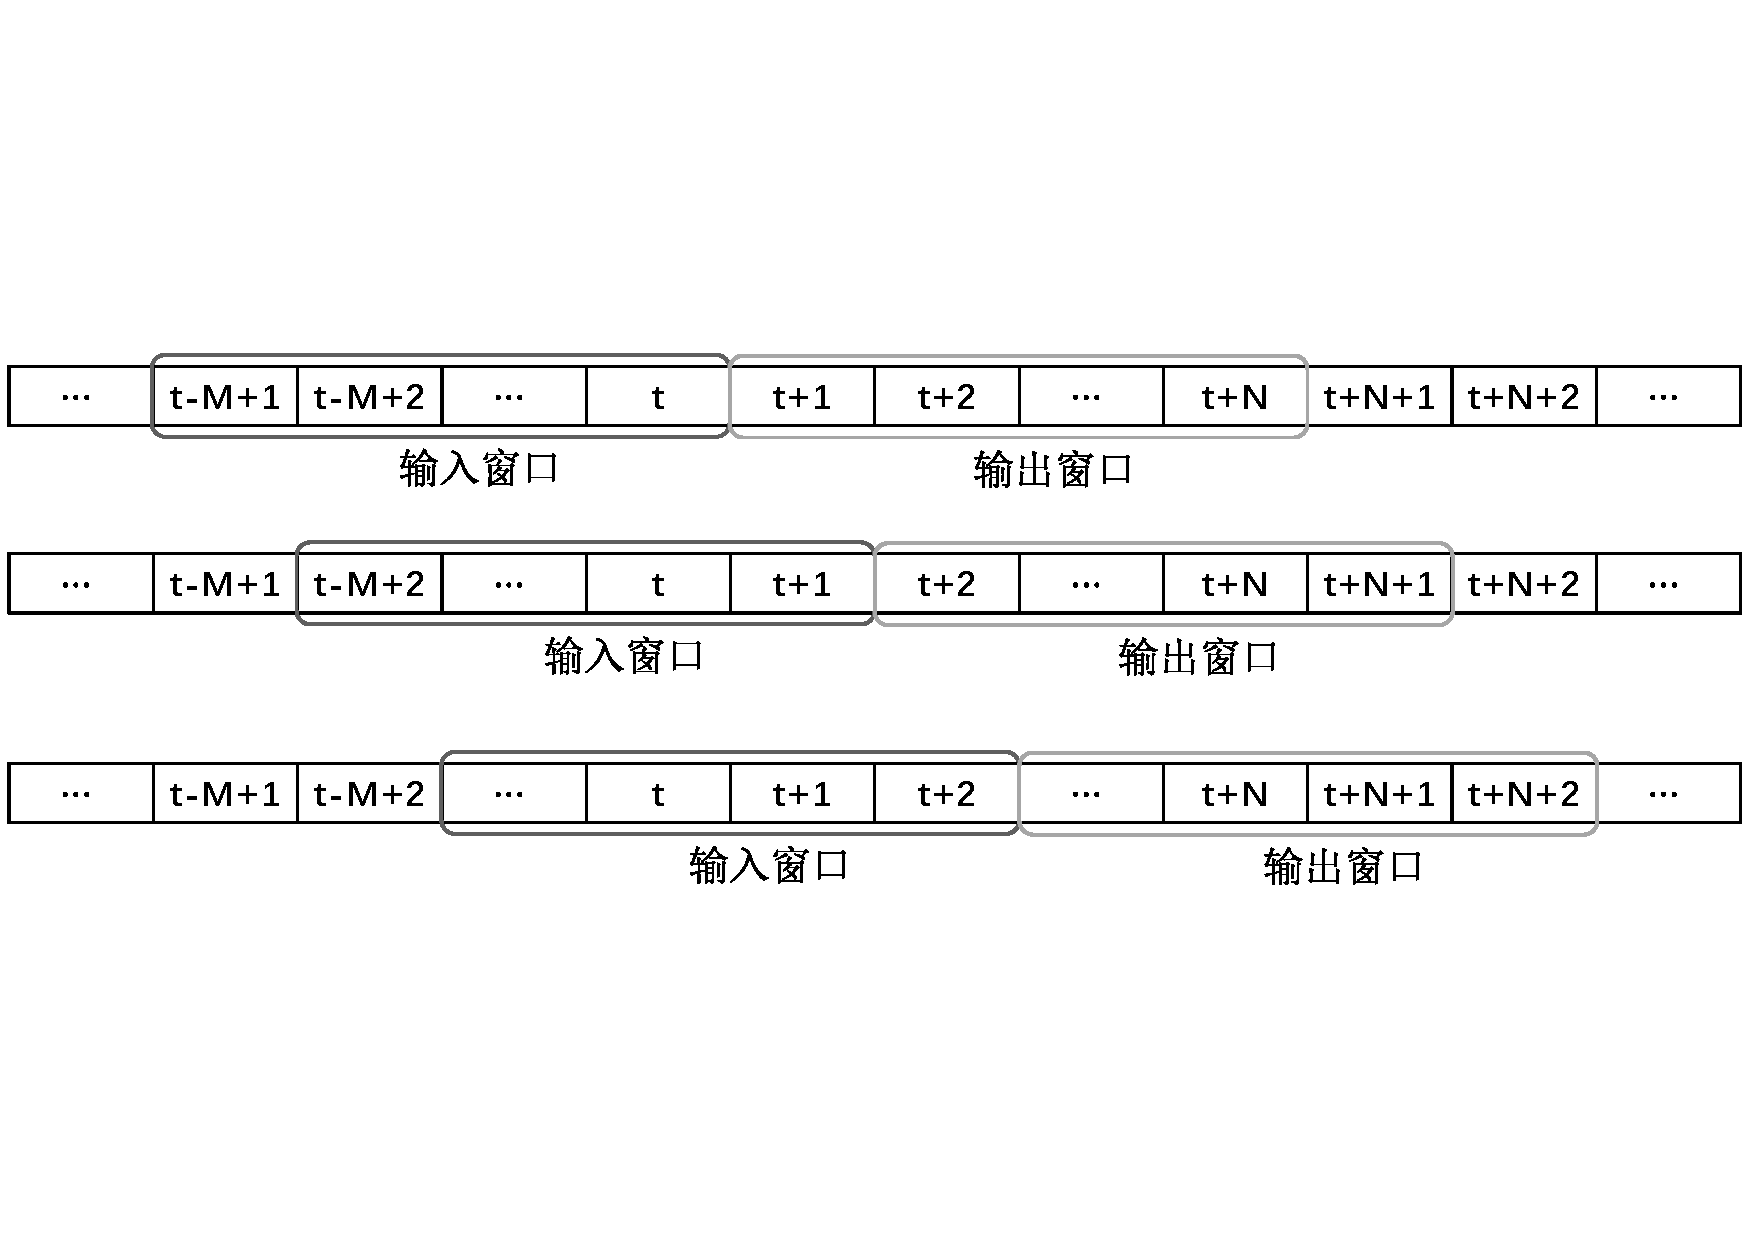
\includegraphics[width=\textwidth]{Img/slide_window.pdf}
    \bicaption{滑动窗口法的过程. 每一行均是是时间序列数据集. 方框中每个数字代表一个时间步. 输入窗口和输出窗口在整个可用的数据集中按月/年滑动。}{The process of the sliding window method. Each row is time series dataset. Each number in the box represents a time step. The input and output windows monthly/yearly slide basis on entire available dataset.}
    \label{fig:slide_window}
\end{figure}

\section{总结}\label{sec:ann_总结}

在本章节中,我们详细介绍了机器学习的理论基础以及相关优化的重要概念和方法。引言概述了以数据驱动的机器学习算法。在第二部分中,通过分别各种机器学习算法的基础理论的数学推导。在第三部分中,说明了模型的优化原理和性能度量标准。近年来,随着机器学习理论的不断推进以及数据处理能力的不断提升,机器学习在地球物理领域的理论建模和数据分析逐渐增多。在未来几年,机器学习会取得更大的发展和进步,给地球物理领域带来更多革命性的发现。